% !TEX program = xelatex
% 编译方式:xelatex 技术文档合集.tex(中文文档,xeCJK 指定 Windows 中文字体)
% 六章合集(与六个分册共享 body_ch1~ch6 正文),封面/摘要/目录 + 六章
\documentclass[11pt,a4paper]{report}
\usepackage[margin=2.4cm]{geometry}
\usepackage{xeCJK}
\setCJKmainfont{SimSun}[BoldFont=SimHei]
\setCJKsansfont{SimHei}
\setCJKmonofont{FangSong}
\setlength{\parindent}{2em}
\usepackage{indentfirst}
\usepackage{booktabs}
\usepackage{array}
\usepackage{enumitem}
\usepackage{amsmath}
\usepackage{graphicx}
\usepackage{float}
\usepackage{needspace}
\usepackage{fancyhdr}
\usepackage{titlesec}
\usepackage{hyperref}
\hypersetup{colorlinks=true,linkcolor=black,urlcolor=blue,
  pdftitle={技术文档——安路 FPGA 双板实时视频系统}}

\titleformat{\chapter}[block]{\centering\LARGE\bfseries}{第\,\thechapter\,章}{0.8em}{}
\titlespacing*{\chapter}{0pt}{-10pt}{26pt}
\renewcommand{\contentsname}{目\hspace{0.5em}录}
\renewcommand{\figurename}{图}
\renewcommand{\tablename}{表}
\setcounter{tocdepth}{2}

\pagestyle{fancy}
\fancyhf{}
\fancyhead[L]{\small 安路 FPGA 双板实时视频系统(相机推流 + HDMI 回显)}
\fancyhead[R]{\small 第\thepage\ 页}

\newcommand{\oneline}[1]{%
  \begin{center}\fbox{\parbox{0.94\textwidth}{\textbf{一句话概括:}#1}}\end{center}}

\begin{document}

% ============================ 封面 ============================
\begin{titlepage}
\centering
\vspace*{2.5cm}
{\huge\bfseries 基于安路 FPGA 的实时图像处理系统\\[8pt]及其在血细胞形态学检测中的应用\par}
\vspace{22pt}
{\LARGE 技术文档\par}
\vspace{36pt}
{\small 全国大学生嵌入式芯片与系统设计竞赛 2026 FPGA 赛道(安路科技)\quad DEMO\par}
\vspace{4pt}
{\small 文档日期:2026 年 10 月 14 日\par}
\vfill
\end{titlepage}

% ============================ 摘要 ============================
\pagenumbering{Roman}
\chapter*{摘要}
\addcontentsline{toc}{chapter}{摘要}

本文档阐述安路 FPGA 双板实时视频系统的设计与实现。相机主板(安路 PH1P35,
MLKPAI-F02)以 SC500CS MIPI 摄像头输入 1280$\times$720@30fps,经自研 ISP——4:1
位宽变换、RAW 域坏点检测与修复(同色对角两级判据)、BGGR 双线性去马赛克与色彩
校正——完成像素处理,并承载自动曝光(AE)与自动白平衡(AWB)两个 3A 闭环
(AWB 回注数字增益帧内生效,AE 以固定点 PID 联合调节传感器曝光与 FPGA 数字增益),提供七种实时
风格化模式后打包为千兆 UDP 码流(1920 包/帧)推流;板内以 128\,bit 公共像素流
接口贯穿算法挂接点。显示子板(安路 EG4D20,MLKPAI-F01)经镜像网口接收同一码流,
由帧重组器完成丢包容忍(缺口白名单、小缺口冻结延展、跟踪-丢弃至下一帧头)与顺序光栅重建,DDR1
三缓冲解耦 30fps 写与 60Hz 读,最终以 HDMI 720p60 实时回显并叠加 OSD。PC 上位机
(Python GUI)收图预览,并经 UDP 6001/6002 命令-状态链路运行时控制曝光、模拟增益
与白平衡。主板当前基线为 v38(PID Q10 系数 6/3/1),自适应两/四帧统计与
曝光优先分配均纳入闭环;42 项 RTL、两组包校验、38 项 Python 回归和 460 帧视频
链路模型通过,当前源码已完成上板验证。布线后 Slice 为 10944/21216 (51.58\%),Setup WNS
+0.119\,ns、Hold WNS +0.020\,ns、TNS 均为 0。v29 曾完成纯资源优化与逐位差分
验证;v30 后主板本地 DDR/DSI 支路已裁剪,ETHB 镜像仍驱动子板 HDMI。显示子板通过 8 场景
记分板、全分辨率逐字节比对与 DDR 仲裁压力扫描等仿真回归并上板验证。文档进一步
给出"级联检测"应用设计:FPGA 实时框选 Giemsa 染色白细胞并裁剪上传,板端 LeNet
轻量网络完成五分类,将商用形态学分析仪"检出—分类"链路中的检出半程移入千元级
国产 FPGA。

\vspace{1em}
\noindent\textbf{关键词:}\ FPGA;MIPI CSI-2;ISP;自动曝光;自动白平衡;坏点检测;
去马赛克;千兆 UDP;帧重组;DDR 三缓冲;HDMI;血细胞形态学检测

\tableofcontents
\clearpage
\pagenumbering{arabic}
\setcounter{page}{1}

\chapter{系统架构}
\oneline{安路 FPGA 双板实时视频系统:相机主板(PH1P35)把 SC500CS 图像经自研 ISP
处理后以千兆 UDP 推流;PC 上位机收图并网络控制曝光/白平衡/模式;显示子板
(EG4D20)接收同一路码流,经帧重组、DDR 三缓冲后输出 HDMI 720p60 实时回显。}

\section{系统概览}

系统由一块相机主板、一块显示子板与 PC 上位机构成(图~\ref{fig:system})。主板
(MLKPAI-F02,安路 PH1P35)完成图像采集、ISP 处理与千兆 UDP 推流,具有两个以太网
口:ETHA 连接 PC 上位机(收图与控制),ETHB 为镜像输出口,输出与 ETHA 完全相同的
RGMII 发送流。显示子板(MLKPAI-F01,EG4D20)从 ETHB 直连网线接收码流,完成协议
解析、帧重组与三缓冲后以 HDMI 720p60 输出到显示器——它是纯接收显示设备,无命令
通路、零参数调节。PC 上位机(Python GUI)经 UDP 6000 收图预览、UDP 6001 下发
曝光/白平衡/模式命令、UDP 6002 接收状态与应答。

\begin{figure}[H]\centering
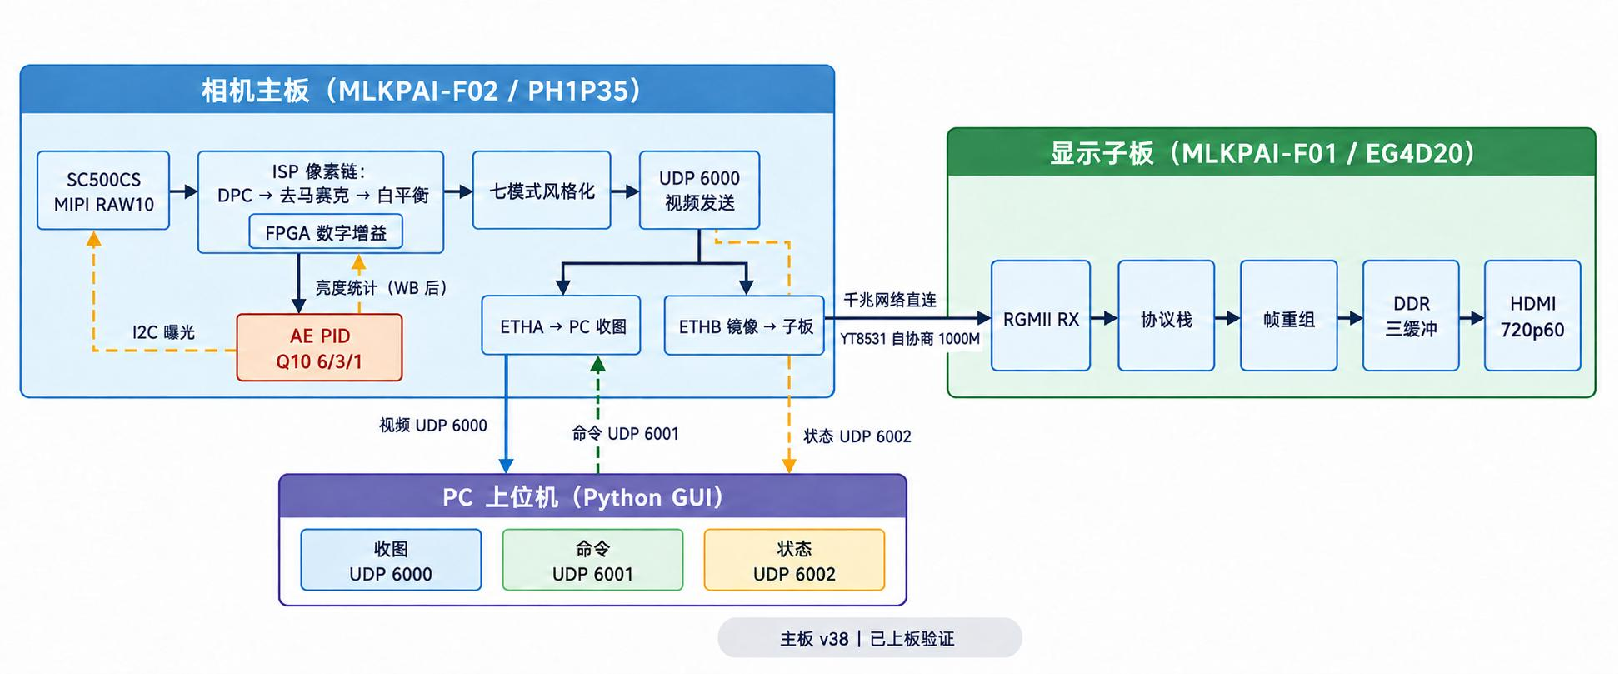
\includegraphics[width=\textwidth]{figs/fig_system.pdf}
\caption{双板系统总览:相机主板、显示子板与 PC 上位机}
\label{fig:system}
\end{figure}

两路显示并行:PC 端预览(ETHA)与子板 HDMI 回显(ETHB)。主板本地 DDR/DSI
显示支路已在 v30 裁剪,7 寸屏背光关闭;网络镜像和相机处理链不依赖该支路。子板
偶发丢包由帧重组器容忍:不超过 4 包的缺口采用最后有效像素冻结延展,更大缺口
跟踪并丢弃至下一帧头,无需重传。主板当前软件基线为 v38
(PID Q10 系数 6/3/1),子板为 v28;当前源码已完成仿真、综合、布线与上板验证。

\section{关键技术指标}

系统的关键技术指标汇总如下表。

\begin{table}[H]\centering\small
\caption{系统关键技术指标}
\begin{tabular}{>{\bfseries}l p{11.2cm}}
\toprule
图像规格 & 1280$\times$720 RGB888;主板采集与推流 30\,fps,子板 HDMI 输出 60\,Hz \\
视频链路 & UDP 6000,每帧 1920 包 $\times$ 1440 字节(480 像素/包),包头 6 字节
(帧序号/格式/4 字节大端偏移);线速约 697\,Mbps(千兆链路必须) \\
命令/状态链路 & UDP 6001 命令(广播,魔数校验);UDP 6002 状态与应答包 \\
网络约定 & 板卡 192.168.1.66;PC 192.168.1.100/24;子板本地 IP 设为流的
目的地址,PC 控制侧不占用该地址 \\
主板器件 & 安路 PH1P35(MLKPAI-F02)+ SC500CS 摄像头模组 + YT8531 千兆 PHY
$\times$ 2 \\
子板器件 & 安路 EG4D20(MLKPAI-F01,EG4D20EG176)+ YT8531 千兆 PHY + 合封
DDR1 16MB \\
板间链路 & 千兆网线直连,两端 YT8531 自协商 1000M \\
上位机 & Python GUI:收图/预览/存帧,曝光、增益、白平衡四模式、算法模式切换 \\
运行验证 & 历史主板七模式 + AE/AWB 连续运行 300\,s,平均 29.965\,fps、
完整率 100\%,无视频流/I2C 错误;该定量板测早于 v38。v38 源码已上板验证,
仿真/综合/布线结果如下:
Setup WNS +0.119\,ns、Hold WNS +0.020\,ns、TNS 均为 0,Slice 10944/21216
(51.58\%)。本文未将早期板测帧率数据误记为 v38 数据。子板全分辨率真机工况仿真(1920 包/帧 $\times$ 11 帧)
逐字节比对通过,上板 HDMI 显示正常 \\
\bottomrule
\end{tabular}
\end{table}

\section{文档组织}

本技术文档按"系统—主板—子板—应用"组织:第 2 章讲主板相机工程的数据通路
(采集解包 $\to$ ISP $\to$ 推流);第 3 章讲 ISP 与图像算法(像素处理链、DPC、
去马赛克、色彩校正与 AWB/AE 两个 3A 闭环、七种风格化模式);第 4 章讲命令通路
与运行时控制(命令解析、I2C 执行通道、手动/自动语义);第 5 章
讲子板 HDMI 回显工程(RGMII 接收、协议栈、帧重组器、DDR 三缓冲、显示输出);
第 6 章讲血细胞形态学检测应用设计。各章自成体系,交叉处以"见第 X 章"互引。

\section{仓库结构}

\begingroup\scriptsize
\begin{verbatim}
CameraVideoPath-on-fpga/
├── README.md                    本文档:系统拓扑、双板工程入口、验证摘要
├── 08_csi_dsi_cs500_7cun/       主板相机工程:MIPI 接收、ISP、风格化、UDP 发送、
│                                上位机脚本、TD 工程、发布说明
├── HDMI_OUT/                    子板 HDMI 回显工程:
│   ├── uisrc/01_rtl/            cvp_hdmi_top(顶层) cvp_rx_assemble(帧重组)
│   │                            rgmii_cdc(跨时钟域) osd_anlogic_logo(OSD)
│   ├── uisrc/03_ip/             复用例程 IP:UDP 协议栈/FDMA/DDR1/VTC/HDMI TX
│   ├── uisrc/04_pin/            引脚与时序约束(pin.adc / timing.sdc)
│   ├── tools/sim/               ModelSim 全链路仿真(Python 向量注入+记分板回归)
│   └── doc/                     架构文档与调试交接
├── releases/                    各版本比特流与发布记录
└── 技术文档/                    本技术文档系列
\end{verbatim}
\endgroup

{\small\sloppy\textbf{说明:}\ 主板与子板工程分别对应独立 TD 工程
(\texttt{camera\_to\_dsi\_display.al} 与 \texttt{HDMI\_OUT.al}),均以 PROGRAM\_SRAM
方式加载(SRAM 断电丢失)。子板复用厂商例程的协议栈、FDMA、DDR 与 HDMI 发送 IP,
其中仅 \texttt{uimac\_rx.v} 有一处有意修改(广播 IP 帧放行),从例程目录重新拷贝
时必须保留该补丁。}

\section{设计原则}

全系统贯彻四条原则。其一,\textbf{流式处理}:主板 ISP 与子板重组器均为无反压流式
流水,常数延迟、按拍处理。其二,\textbf{接口标准化}:主板内部以 128\,bit 公共像素
流接口(CVP\_PIXEL\_V1,含坐标/帧身份/模式号元数据)贯穿算法挂接点,即插即用。
其三,\textbf{验证闭环}:v38 的 42 项 RTL、两组网络包校验、38 项 Python
回归与 460 帧视频链路模型通过;v29 资源优化的 22 项回归(含新旧实现同激励逐位差分对照)、子板 8 场景记分板
与全分辨率逐字节比对等仿真均通过,当前源码已完成上板验证。其四,\textbf{约束显式化}:两板
的时钟组、采样相位与带宽预算全部显式声明并留余量(子板 DDR1 带宽占峰值 55\%)。

\chapter{主板相机工程:采集与推流}

\section{主板数据通路总览}

主板把 SC500CS 传感器图像处理为千兆 UDP 码流,ETHB 镜像到显示子板(图~\ref{fig:mainboard})。主链路:SC500CS(MIPI 2lane RAW10,采窗
1287$\times$727,实发 1280$\times$720)$\to$ csi\_unpacket/raw10 解包 $\to$
uial2axis $\to$ line\_retimer(重切 320 拍 $\times$ 720 行)$\to$ group\_fifo
(40.2M $\to$ 100M 跨时钟域)$\to$ cvp\_proc(4:1 位宽变换 + DPC + 去马赛克,
见第 3 章)$\to$ color\_correct(白平衡)$\to$ 七模式风格化 $\to$ pack\_4(攒
96\,bit 组)$\to$ cvp\_eth\_dbg(GMII 125\,M 域字节展开)+ cvp\_gmii\_mac\_tx
$\to$ RGMII $\to$ YT8531 PHY $\to$ ETHA(PC)与 ETHB(镜像,子板)。

\begin{figure}[H]\centering
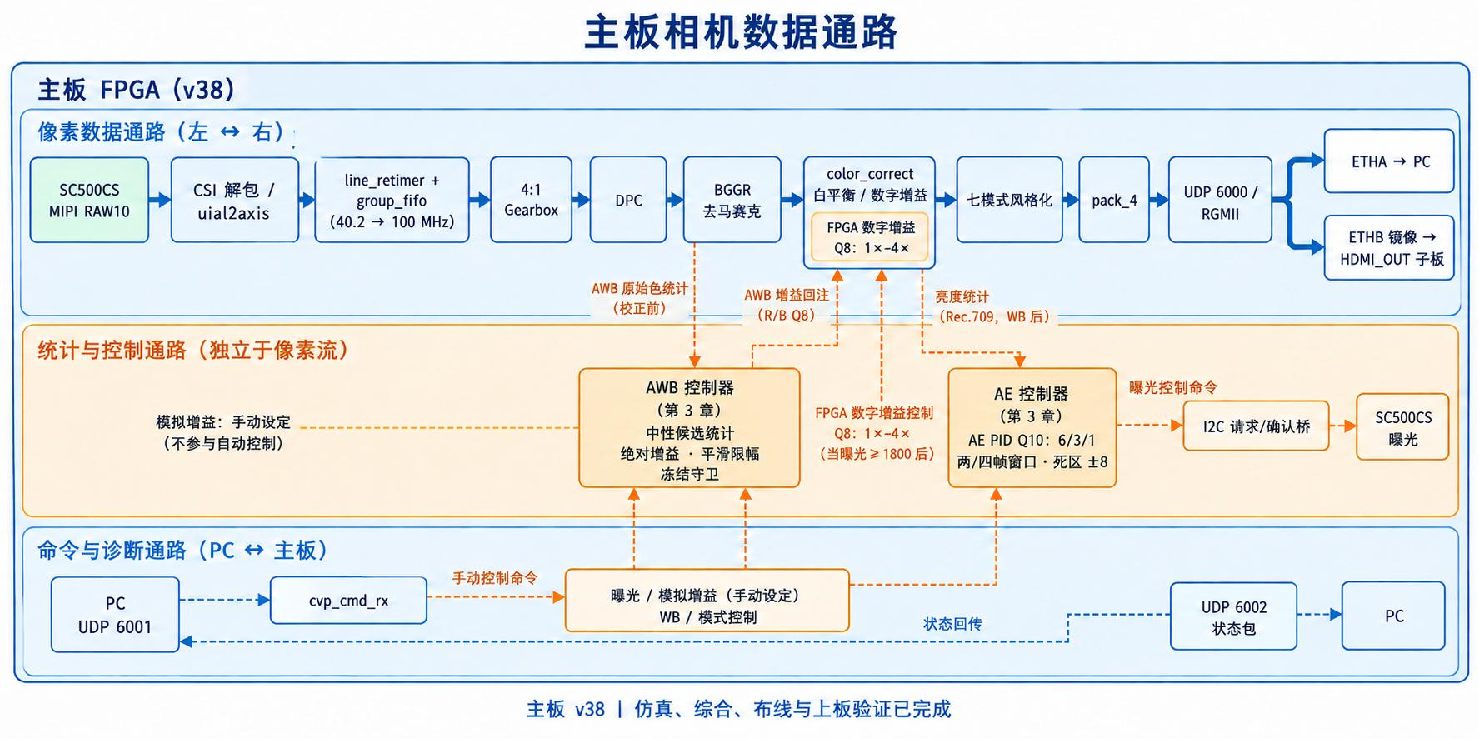
\includegraphics[width=\textwidth]{figs/fig_mainboard.pdf}
\caption{主板数据通路:采集解包 / ISP / 推流 + 命令与状态支路}
\label{fig:mainboard}
\end{figure}

\section{采集与解包层}

采集层负责三件事:传感器配置、MIPI 字节流还原、行帧切分与跨时钟域。传感器工作
参数由 \verb|uics500_cfg/| 配置表(主表/AE 表/SC500GainTbl 增益表,档位 16..143
= 1.0$\times$..15.75$\times$)经 I2C 写入,时序由 uicfgcs500 状态机控制。定版
关键值:VTS=1003 行(30.0\,fps 实测校准);采窗 1287$\times$727 居中于原 1080p
窗,实发 1280$\times$720;默认曝光 500 半行、合法范围 62..1800——曝光上限的原因
是贴近满帧时传感器读出窗相对帧同步偏移数行,720 行窗口的顶部或底部会出现错位带,
1800(900 行)留 103 行裕量;需更亮优先加增益档或补光。

\textbf{行帧切分}:\verb|uial2axis| 整理为 AXI-Stream 并做行/帧切分;
\verb|line_retimer| 把流重切为 320 拍 $\times$ 720 行的规整节拍。这一级有两个
关键实现约束:采窗行数(727)与实发行数(720)是两个不同的参数,不可混淆——用错
会造成帧头漂移、上下半帧互换;行列计数必须与帧起始对齐,否则去马赛克的色平面会
错位。\textbf{跨时钟域}:\verb|group_fifo| 以异步 FIFO 完成 40.2\,MHz 采集域到
100\,MHz 主域的衔接,并统一组格式——下游齿轮箱按"40\,bit(4 像素)/拍"消费,
每拍拿到完整一组。

\textbf{采集健康度}由网口状态上报直接观测(v29 起串口诊断链已移除,由 UDP 6002
状态包替代):状态包含帧计数、组数、流错误与 I2C 诊断,GUI 状态栏实时显示 fps 与
完整率。判定基准:$f=30$、每帧 230{,}400 组;GUI 能收图即采集到推流全链路健康,
收不到图先排查 PC 侧 6000 端口占用(多进程分流是假读数的根源),仍无图再看状态包
帧计数是否走动。摄像头启动带等待与重试机制,并以"第一完整帧"门控后续处理,上电
即出流无需手动干预。

\section{推流层:千兆 UDP 发送}

推流层把 RGB888 像素流打包为千兆 UDP 码流。\verb|pack_4| 攒 4 像素 96\,bit 组;
\verb|cvp_eth_dbg| 在 GMII 125\,MHz 域做字节展开,按\textbf{每帧 1920 包、每包
1440 字节(480 像素)}发送;应用头 6 字节(帧序号、格式字节、4 字节大端偏移 =
包序 $\times$ 1440);以太网帧 1500 字节(ETH14 + IP20 + UDP8 + 头 6 + 数据
1440 + FCS4),目的 MAC 广播、目的 IP 192.168.1.100、端口 6000/6000(状态包
6002)。带宽核算:1920 包 $\times$ 12\,$\mu$s $\approx$ 23.6\,ms/帧 $\to$
30\,fps,线速约 697\,Mbps——必须千兆链路,100M 下必然丢流。

ETHA 与 ETHB 共享同一发送通路,ETHB 输出与 ETHA 完全相同的 RGMII 流(镜像口),
因此 PC 预览、子板回显与状态上报天然一致;两颗 YT8531 各自与对端自协商 1000M。

\section{公共像素流接口(CVP\_PIXEL\_V1)}

风格化与分类挂接点采用统一的 128\,bit 像素字接口:RGB888(23:0)、x/y 坐标
(12 位零起始)、32 位采集帧身份、16 位配置号、8 位模式号、SOF/EOL/EOF 标志
(与对应像素同拍)、错误指示与 OSD/AE/WB 状态位,时钟复位单独传递。摄像头分支
无反压(禁止任意 backpressure),每帧恰 921{,}600 个有效像素、720 个行尾与一个
帧尾。RGB 窗口边界复制、RAW Bayer 窗口反射(保持同色相位)。接口约定保证了点
运算的 RGB 延迟与元数据一致、窗口算子的输出坐标代表实际窗口中心——任何新算法
模块(如分类网络)按此接口即可挂接,不动主链路。

\section{主板显示支路裁剪与状态上报}

v30 起主板移除本地 DDR 帧缓存、显示裁剪与 DSI 发送链,并关闭 7 寸屏背光;
相机、ISP、AE/AWB、UDP 发送、命令接收和状态上报保持工作。ETHB 与 ETHA
仍是同一路 RGMII 发送流的镜像,子板 HDMI 回显因此不依赖主板本地显示硬件。
状态经 UDP 6002 回传,帧计数、RAW 组数、输出长度、I2C 与流错误可供 GUI 诊断。

\section{资源优化与版本状态}

v29 的五项资源优化与差分验证记录如下,作为历史基线;之后 v30 裁剪本地 DDR/DSI
支路,v31--v38 继续更新算法、流恢复与 AE 控制器。当前主板源码为 v38,并非 v29
资源快照。PH1P35MDG324、TD 6.2.168116、100\,MHz 图像时钟的 v38 布线结果为:

\begin{center}\small
\begin{tabular}{lr}
\toprule
指标 & v38 主板版本 \\
\midrule
Slice & 10944 / 21216 (51.58\%) \\
LUT6 / FF & 8807 / 11035 \\
ERAM20K & 51 / 108 \\
DSP & 16 / 40 \\
PLL & 2 / 6 \\
Setup WNS / Hold WNS & +0.119\,ns / +0.020\,ns \\
Setup TNS / Hold TNS & 0 / 0 \\
\bottomrule
\end{tabular}
\end{center}

v38 的 RTL/包校验/Python 回归与 460 帧视频链路模型均通过,当前源码已上板验证。
上表为综合布线报告;AE 控制器仿真对比与板级观测分别记录,本文不把仿真响应当作
板测指标。以下为历史 v29 数据:

主板工程在功能定版(v27)后做了一轮纯资源优化(v29),为应用章的 LeNet 分类网络
腾挪空间,全部改动经新旧实现\textbf{同激励逐位差分}验证,功能与接口不变:

\begin{enumerate}[nosep]
\item \textbf{统计直方图 LUTRAM 化}(cvp\_frame\_stats):32 箱亮度直方图由触发器
阵列改为分布式 RAM,消隐期旋转清扫,走查直读——模块触发器 2312$\to$1044,
F7/F8 多路器清零;
\item \textbf{状态跨域链 ERAM 化}:原 1536\,bit 状态字经三份寄存器跨域传递改为
双 bank ERAM 快照 + 发送期流式读,线上字节序与原实现位精确;
\item \textbf{元数据 FIFO 寄存器化}(风格化/轮廓支路):帧原子元数据的小队列改单
寄存器,腾出 2 块 ERAM20K;
\item \textbf{数据通路摘异步复位}:纯数据延迟链去复位、控制类寄存器保留,统一
触发器控制集;
\item \textbf{移除串口诊断链}:帧率/健康判定改由 UDP 状态包覆盖(见 2.2 节)。
\end{enumerate}

布线结果:Slice 从 17359 降至 15006 (81.8\% 降至 \textbf{70.7\%}),触发器
从 19999 降至 15462 (减少 23\%),LUT 从 14455 降至 12744,ERAM 从 66 降至 65;
Setup WNS +0.102\,ns、Hold WNS +0.020\,ns、TNS 0。回归 22 项全过(v26 套件 12 + v27 套件 6 +
差分 4:统计 17 帧、风格化 14 帧全输出逐位一致,状态链线上包含 CRC 逐字节比对)。

\chapter{ISP 与图像算法}
\oneline{ISP 层由像素处理链与两个统计-控制闭环组成:4:1 位宽变换 $\to$ DPC 坏点
修复 $\to$ 去马赛克 $\to$ 白平衡/数字增益的流式像素链,叠加 AWB 增益回注与
v38 自动曝光 PID——AE 经 I2C 调节传感器曝光,达到上限后调节 FPGA 数字增益,
模拟增益保持手动;再加七种实时风格化模式。本章给出原理、判据与验证。}

\section{ISP 流水与 3A 闭环}

ISP(Integrated Signal Processing)层完成"RAW10 像素组 $\to$ 校色后 RGB888 流"
的全部处理,并承载经典 3A 闭环中的两个——自动曝光(AE)与自动白平衡(AWB)。
整体结构如图~\ref{fig:isp3a} 所示:\textbf{像素处理链}为流式流水(4:1 位宽变换
gearbox $\to$ DPC $\to$ 去马赛克 $\to$ color\_correct,全部常数延迟);两个
\textbf{统计-控制闭环}的口径刻意分离——AWB 在\textbf{校正前}的 RGB 上估计
传感器原始色偏,AE 在\textbf{校正后}的图像上测亮度(与输出画面同口径)。
AWB 闭环把算出的绝对增益回注 color\_correct(下一帧生效);v38 AE 闭环把曝光码
经 I2C 请求/确认桥写入传感器,触及曝光上限后在像素域提高数字增益(1$\sim$4 倍);
模拟增益保持手动设定。网络手动命令可随时接管
任一闭环(见第 4 章)。

\begin{figure}[H]\centering
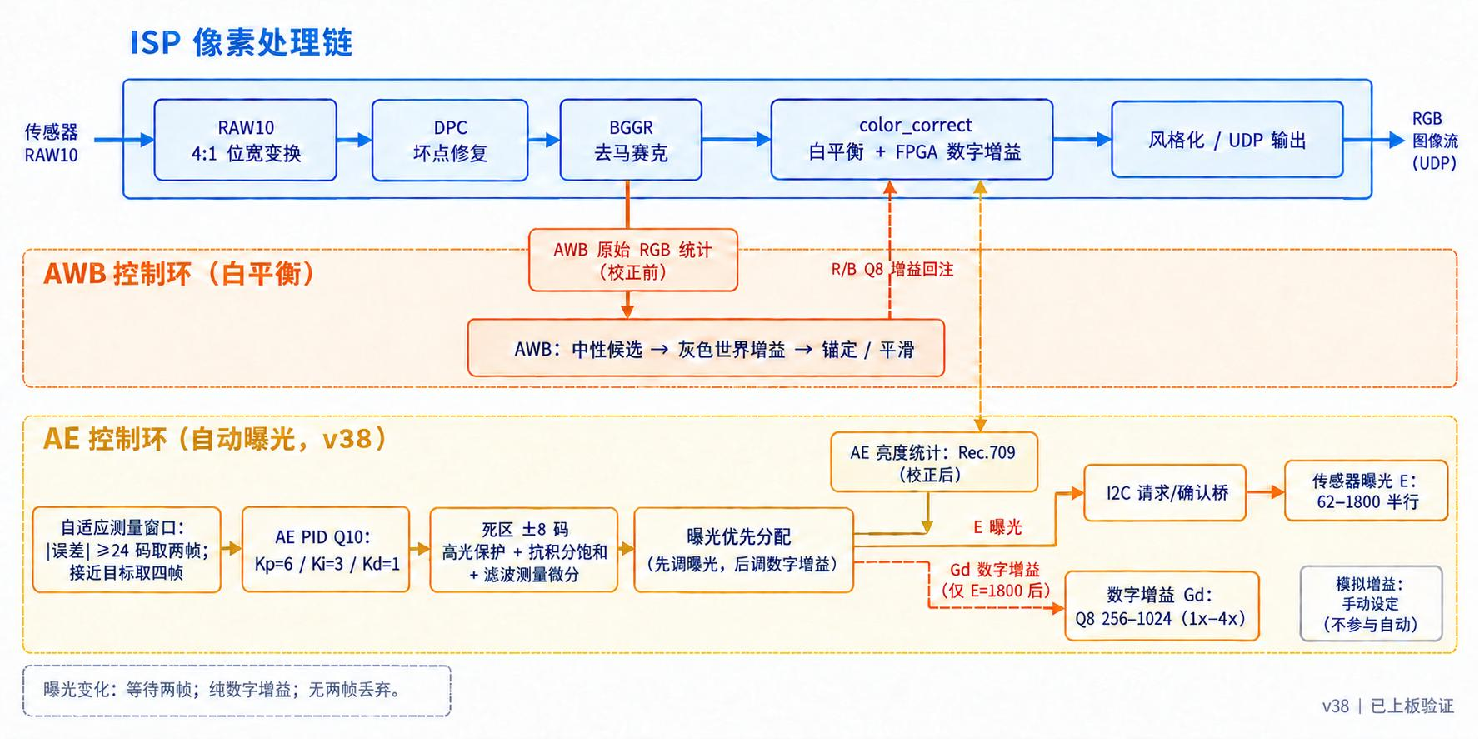
\includegraphics[width=\textwidth]{figs/fig_isp_3a.pdf}
\caption{ISP 层与 3A 闭环:像素处理链(实线)与 AE/AWB 统计-控制回路}
\label{fig:isp3a}
\end{figure}

\section{坏点检测与修复:RAW 域同色对角判据(DPC)}

坏点(sensor 出厂缺陷或高增益下的离群像素)若留到彩色重建之后才处理,一个坏点会经
双线性插值扩散成 5 像素的十字彩色斑;因此 DPC 插在位宽变换之后、去马赛克之前的
RAW10 域,此时一个坏点只是一个孤立的 10\,bit 值,处理代价最小。

\textbf{判据:}Bayer 排列下,$3\times3$ 窗口内与中心同色的恰是 4 个对角点
($d_1=p_{00}$、$d_2=p_{02}$、$d_3=p_{20}$、$d_4=p_{22}$)——这对任何 CFA 相位都
成立,无需相位信息。坏点的本质是"与所有同色邻居同时、同向、不连续地偏离",据此
两级判据:
\begin{align*}
\text{亮点坏点:}\quad & c>\max_i d_i+\mathrm{TH}\quad\text{且}\quad c>\overline{d}+\mathrm{TH}_2;\\
\text{暗点坏点:}\quad & c+\mathrm{TH}<\min_i d_i\quad\text{且}\quad c+\mathrm{TH}_2<\overline{d},
\end{align*}
其中 $\overline{d}=\frac{1}{4}\sum_i d_i$。只看 max/min 单阈值会把噪声尖峰误判成
坏点(高增益时尤甚),与均值的偏离量能滤掉大部分噪声;而"四个邻居全部同向偏离"
本身也抗纹理误检——细线、边缘上邻居一亮一暗、方向不一致,不会触发。

\textbf{矫正:}命中才把中心替换为 4 个同色邻居的中位数,其余像素原样直通——与全局
中值滤波的本质区别是只动被判定的像素,不伤分辨率。中位数与 max/min 共用同一级
sort4 部分网络(5 个比较器)。判据与矫正采用两级流水:第 1 拍寄存 sort4 输出与
4 邻居均值,第 2 拍只做阈值加法、比较与矫正选择,满足 100\,MHz 时序;整级固定
4 拍。两处边界选择"不矫正"(宁漏勿错):复制边界处邻居与中心等值时判据自然失效;
每行第 1 个输出槽位的中心落在第 0 列,其"水平邻居"是上一行行尾回绕像素,用列
计数识别并直接旁路。

\textbf{验证:}单元自检注入坏点全部按邻居中位数修复、平滑背景零误检、随机纹理下
与 golden 参考模型逐位一致;全量联合仿真注入亮暗坏点 24 个,24/24 修复、邻域残差
全 0,坏点趟 vs 干净趟全帧 PSNR 101.09\,dB。放大图直观显示:单像素 RAW 坏点经
插值会变成彩色伪影,DPC 修好后输出与干净趟完全一致——坏点必须在 RAW 域、去马赛克
之前修的实证。

\section{去马赛克:BGGR 双线性彩色重建}

Bayer 原始数据的每个像素只携带单一颜色分量,必须插值出全彩;插值相位必须与传感器
的 Bayer 排列严格一致。记 $3\times3$ 窗口及其中心像素为
\begin{equation*}
W=\begin{pmatrix}p_{00}&p_{01}&p_{02}\\ p_{10}&p_{11}&p_{12}\\ p_{20}&p_{21}&p_{22}\end{pmatrix}
\qquad\text{中心像素 }p_{11},
\end{equation*}
插值输出记 $(\hat R,\hat G,\hat B)$,则四种相位为
\begin{align*}
B\text{ 中心:}\quad & \hat B=p_{11},\quad \hat G=\tfrac{1}{4}\bigl(p_{01}+p_{21}+p_{10}+p_{12}\bigr),\quad \hat R=\tfrac{1}{4}\bigl(p_{00}+p_{02}+p_{20}+p_{22}\bigr);\\
R\text{ 中心:}\quad & \hat R=p_{11},\quad \hat G=\tfrac{1}{4}\bigl(p_{01}+p_{21}+p_{10}+p_{12}\bigr),\quad \hat B=\tfrac{1}{4}\bigl(p_{00}+p_{02}+p_{20}+p_{22}\bigr);\\
G\text{ 中心(偶行):}\quad & \hat G=p_{11},\quad \hat R=\tfrac{1}{2}\bigl(p_{01}+p_{21}\bigr),\quad \hat B=\tfrac{1}{2}\bigl(p_{10}+p_{12}\bigr);\\
G\text{ 中心(奇行):}\quad & \hat G=p_{11},\quad \hat B=\tfrac{1}{2}\bigl(p_{01}+p_{21}\bigr),\quad \hat R=\tfrac{1}{2}\bigl(p_{10}+p_{12}\bigr).
\end{align*}
即已知色取自身,缺失色分别用同色正邻域均值或对角均值插值;输出 8\,bit 取 10\,bit
结果的高 8 位。固定 3 拍延迟、复制边界(首行首列同样正确)。一处关键标定:数据到达
时行相位比 BGGR 排列假设差一整行,因此行偶判定使用行计数低位本身——该相位以色块
自检(灰底放置红/绿/蓝/白块,逐行核对输出颜色)确认;行列计数与帧起始的对齐保证
色平面不错位。

\section{色彩校正与自动白平衡(AWB)}

color\_correct 在去马赛克之后完成白平衡,每像素校正为
\begin{equation*}
O_c=\min\bigl(255,\ \mathrm{round}(I_c\,g_c/256)\bigr),\qquad c\in\{R,B\},\quad g_G\equiv 256,
\end{equation*}
即 Q8 定点乘法(8$\times$9\,bit 取高位、四舍五入、饱和到 255),$G$ 通道锚定
1.0$\times$——Von Kries 形式只调色温不漂移亮度;另支持全模式 R/B 通道互换
(色序错配一键修)。白平衡有四种工作模式:\textbf{标定预设}(出厂标定增益,
R344/G256/B451)、\textbf{色温 K 值}(拖动色温 2500$\sim$10000\,K,经光源近似
曲线换算 R/B 增益,6500K 为参考锚点)、\textbf{手动 RGB}(Q8 增益
64$\sim$1024,256 = 1.0$\times$)与\textbf{自动场景(AWB 闭环)}。

\textbf{AWB 闭环}是 ISP 的统计-控制回路,统计在\textbf{未校正}的 RGB(去马赛克
输出、数字增益之前)上进行——估计的是传感器原始色偏,不受当前增益影响;闭环
每帧执行四步:

\textbf{(1) 中性候选判据。}先把三通道按标定先验加权
\begin{equation*}
R'=\tfrac{344}{256}\,R,\qquad G'=G,\qquad B'=\tfrac{451}{256}\,B,
\end{equation*}
在先验拉平后的色度上判中性。宽松判据为
\begin{equation*}
2\bigl(\max_c C'_p-\min_c C'_p\bigr)\le\max_c C'_p,\qquad
32<Y_p<230,\qquad 2<I_{c,p}<250,
\end{equation*}
即色度散布不超过最大通道的一半、亮度与各通道都在非黑非削顶的窗内。保守判据
(现行配置)收紧为 $8(\max-\min)\le\max$(散布 $\le$ 1/8)外加亮度窗
$64\le G\le224$、$\max<235$、$\min>32$,并要求\textbf{四象限多样性}:画面四等分,
每象限中性样本 $\ge WH/2000$,至少 2 个象限有效才接受本帧估计(防单一物体
主导统计);象限 $\ge$3 且 $n\ge 5\%\,WH$ 判为强置信。

\textbf{(2) 接受条件与冻结守卫。}全帧统计完整(样本数 $=WH$)、中性样本数
$n\ge\max(WH/100,16)$、$\sum_{\mathcal N}R$ 与 $\sum_{\mathcal N}B$ 非零且象限
足够;任一不满足即\textbf{冻结}当前增益并上报原因码(暗场/过曝/样本不足/
象限不足)——宁可不校,不可误校。

\textbf{(3) 增益生成。}对中性样本集 $\mathcal N$ 以 $G$ 为基准求灰色世界增益,
帧尾以 Q8 定点除法完成:
\begin{equation*}
g_R^{\mathrm{cand}}=\mathrm{clip}_{[128,\,1024]}\Bigl(\frac{\sum_{p\in\mathcal N}G_p}{\sum_{p\in\mathcal N}R_p}\Bigr),\qquad
g_B^{\mathrm{cand}}=\mathrm{clip}_{[128,\,1024]}\Bigl(\frac{\sum_{p\in\mathcal N}G_p}{\sum_{p\in\mathcal N}B_p}\Bigr),
\end{equation*}
自动模式限幅 $0.5\times\sim4\times$。

\textbf{(4) 先验锚定与时域平滑。}保守模式下候选先夹到标定基准
$g_{\mathrm{base}}$(R344/B451)的 $\pm25\%$ 邻域再与之混合,随后与当前增益做
一阶惯性平滑:
\begin{align*}
\text{锚定:}\quad & \hat g=\mathrm{clip}\bigl(g^{\mathrm{cand}},\
[\tfrac34 g_{\mathrm{base}},\ \tfrac54 g_{\mathrm{base}}]\bigr),\qquad
g^{\mathrm{mix}}=\begin{cases}\tfrac12\bigl(g_{\mathrm{base}}+\hat g\bigr), & \text{强置信}\\[2pt]
\tfrac14\bigl(3g_{\mathrm{base}}+\hat g\bigr), & \text{弱置信}\end{cases};\\[4pt]
\text{平滑:}\quad & g^{(t)}=\begin{cases}
\bigl(3g^{(t-1)}+g^{\mathrm{mix}}+2\bigr)\gg 2, & \text{宽松模式}\\[2pt]
\bigl(15g^{(t-1)}+g^{\mathrm{mix}}+8\bigr)\gg 4, & \text{保守模式}\end{cases}
\qquad(g_R,g_B\ \text{各自独立}) .
\end{align*}
两级设计让单帧统计噪声只占 1/4(宽松)乃至 1/16(保守)的权重:静态场景增益
快速锁死不振荡,真实色偏仍稳定收敛;实测固定场景自动增益收敛于标定值
(R344/G256/B451)。自动模式不显示伪造的"测得色温"。模式切换与增益设置均经
网络命令运行时生效(见第 4 章),预览与保存图均为正确 RGB 顺序。

\section{自动曝光(AE):固定点 PID 与曝光优先分配}

当前 v38 版本的 AE 采用帧事件驱动的固定点 PID。控制器测量白平衡校正后的 RGB
亮度(与输出图像口径一致),每帧统计亮度均值和高亮像素数;空统计帧不参与控制。
目标默认值为 112,以实际状态包回报的目标为准。高亮像素比例超过 5\% 时启用
高光保护:目标可按当前均值下调并保持,避免控制器在高反差场景中一边压高光、一边
试图抬升全帧均值。高光条件解除且亮度明显偏离时,目标恢复默认值。

测量采用自适应窗口:误差绝对值达到 24 个亮度码时使用最近两帧平均,接近目标时
累计四帧平均。目标死区为 $\pm8$ 码。误差、积分和测量微分均在 Q2 亮度单位中
计算;误差反向时清除积分与微分历史。积分限幅为 $[-512,512]$,对控制输出限幅并
使用抗积分饱和。默认 PID 系数为 Q10 编码 $K_p=6$、$K_i=3$、$K_d=1$,实际
乘数分别为 $6/1024$、$3/1024$、$1/1024$。微分项采用测量微分并作一阶平均:
\begin{equation*}
D_{raw}=\bar Y_{t-1}-\bar Y_t,\qquad
D_t=\frac{D_{t-1}+D_{raw}}{2},\qquad
C=\operatorname{clip}_{\pm C_{max}}\left(\frac{K_pe+K_iI+K_dD_t}{4\cdot1024}\right),
\end{equation*}
其中误差达到 24 码时 $C_{max}=256$,接近目标时为 64;微分项可以抑制
或暂缓调整,但不能使执行方向与当前误差相反。实际硬件内部保留 Q2 精度并按流水
阶段完成运算。

控制器调节总曝光量 $U=E\,G_d$,其中 $E$ 为传感器曝光半行码、$G_d$ 为 Q8
FPGA 数字增益。每次更新按 PID 输出比例改变 $U$,最小变化量为 $1\times256$
(Q8 单位),随后按如下优先级分配:
\begin{align*}
E&\in[62,1800],\qquad G_d\in[256,1024]\quad(1\times\sim4\times);\\
U\le1800\times256&\Rightarrow G_d=256,\quad E\approx U/256;\\
U>1800\times256&\Rightarrow E=1800,\quad G_d\approx U/1800.
\end{align*}
因此先用曝光,触及安全上限后才增加 FPGA 数字增益;模拟增益保持用户手动设定。
曝光上限仍由传感器接近满帧时的读出窗偏移限制,原因见第 2 章。亮度变暗时
数字增益放大噪声,故暗场质量仍需实机评估。

执行采用请求/确认互斥。曝光写入成功后保留两帧稳定保护;纯 FPGA 数字增益在
SOF 锁存,确认帧已经是新增益图像,因此不再丢弃两帧。手动事务会清空旧 PID
历史。6/3/1 闭环模型在亮场和暗转亮场比冻结的 4/1/0 控制器更快,暗场相同、
极暗场略慢;稳定窗口与交替亮度检查无反复调节,460 帧完整视频 RTL 链路模型
通过。上述为仿真对比结论;v38 源码已上板验证,具体板级 AE 响应以对应实测记录为准,
不将仿真差异当作板测指标。
\section{七模式风格化算法}

风格化级以公共像素流接口挂在白平衡之后、推流之前,提供七种实时模式,板上由两个
功能键切换(下一模式/上一模式,切换在帧首生效,状态文字与画面同帧):

\begin{table}[h!]\centering\small
\caption{七种风格化模式}
\begin{tabular}{clp{9.8cm}}
\toprule
模式 & 名称 & 实现 \\
\midrule
0 & 原图 & 白平衡结果直通 \\
1 & 灰度 & $Y=(R+2G+B)\gg2$ 三通道同值 \\
2 & 二值化 & 亮度与阈值比较 \\
3 & Sobel 边缘 & 亮度梯度 $|G_x|+|G_y|$,独立高低阈值双门限 + 滞后连接;
低阈值默认联动为高阈值一半,可解除;两模式参数各自记忆,复位恢复默认 \\
4 & 卡通 & 中值滤波(保边平滑)$\to$ 每通道 3 位颜色量化 $\to$ 黑描边 \\
5 & 素描 & 白底黑线,与边缘共用判决,独立阈值与线宽(加粗) \\
6 & 复古暖色 & 定点 sepia 矩阵变换 \\
\bottomrule
\end{tabular}
\end{table}

边缘与素描的高低阈值、线宽经 GUI 实时可调(如边缘推荐低 45/高 90,素描低 50/
高 100;主阈值越低细节越多);模式切换经帧首生效保证无撕裂。全部模式与 Python
位级参考对拍,并参加七模式轮换长时间运行验证(平均 29.965\,fps、完整率 100\%)。

\chapter{命令通路与运行时控制}
\oneline{上位机经 UDP 6001 广播命令,cvp\_cmd\_rx 在 RGMII 域极简解析后送入
100M 域命令寄存器;手动曝光/模拟增益经 I2C 请求/确认桥写入传感器,AE 则调节
传感器曝光与 FPGA 数字增益;白平衡增益即时覆盖 color\_correct,状态经 UDP 6002
回传。本章讲命令基础设施与手动/自动
切换语义——AE/AWB 闭环的算法本体见第 3 章。}

\section{命令通路:cvp\_cmd\_rx}

cvp\_cmd\_rx 直接在 RGMII 接收域做极简 UDP 命令解析,不经过协议栈:IDDR 还原
字节流 $\to$ 过滤状态机逐条校验(SFD、EtherType=IPv4、协议=UDP、目的端口 6001、
魔数 C5A55001,任一不符即丢帧)$\to$ 命令事件跨时钟域 $\to$ 100\,MHz 域命令寄存器
组。设计上有意不校验 MAC/IP 地址(命令走广播),宽容上位机与脚本混用。

命令域覆盖:曝光码(半行编码)、模拟增益档、白平衡三通道增益(Q8)与模式
(预设/色温 K/手动/自动)、R/B 互换、算法模式与阈值参数。手动曝光/模拟增益经
I2C 桥重写传感器(约 1$\sim$2 帧生效);白平衡增益直接覆盖 color\_correct
(即拖即生效)。自动曝光由 PID 控制器优先调整传感器曝光,到达上限后调节 ISP
中的 Q8 数字增益;模拟增益保持用户设定。状态与应答包经 UDP 6002
回传(含 CRC 与 IPv4 校验和)。

\section{I2C 请求/确认桥:传感器曝光执行通道}

传感器寄存器写入(上电初始化、AE 曝光更新与手动设置)共用单一的请求/确认桥:任何时刻
只有一个在飞的写事务,写入中的数据保持不变,I2C 异常以 NACK/超时上报到状态口。
这一设计同时服务初始化和运行期写入——初始化按配置表(主表/AE 表/增益表)批量写入,
运行期由手动命令更新传感器曝光码与模拟增益档,AE 闭环(第 3 章)则通过该桥更新
曝光码,并在像素处理域独立锁存数字增益;自动控制不改写模拟增益档。摄像头启动流程带
等待与重试,并以第一完整帧门控后续流水,上电即出流无需手动干预。

\section{手动/自动切换语义}

GUI 与命令行的操作语义固定:拖动曝光或模拟增益即关闭自动曝光转入手动;拖动 RGB
增益即切换手动白平衡;自动模式下的参数写入同样走确认应答。GUI 显示的是确认写入
的值——界面不声称读回了传感器寄存器,传感器生效可能延后数帧。边缘/素描的阈值
参数与算法模式切换同属命令域,切换在帧首生效、无撕裂。

\section{状态与诊断}

运行状态经两个通道可观测:UDP 6002 状态/应答包(GUI 实时显示写入确认、I2C 健康、
帧计数与流错误;v29 起并承担链路健康判定——GUI 能收图即全链路正常,收不到图先排查
PC 侧 6000 端口占用)与 GUI 状态栏(fps 与完整率,正常 100\%)。测量纪律:UDP 抓帧
必须独占 6000 端口(只打开一个收图程序),否则端口分流会产生假读数。

\chapter{子板 HDMI 回显工程}

\section{职责与数据通路}

显示子板(MLKPAI-F01,EG4D20EG176)是纯接收显示设备:从主板 ETHB 镜像口接收
千兆视频码流,还原为 1280$\times$720 图像后以 HDMI 720p60 实时输出。板上无命令
通路、零参数调节;协议栈发送侧请求恒为零(纯二层接收,ping 不通属正常)。数据
通路按三个时钟域组织(图~\ref{fig:subboard}):\textbf{clk\_125} 域完成 RGMII
接收(PLL2 控制采样相位 + IDDR)、rgmii\_cdc 跨域、MAC/IP/UDP 协议栈解析与帧
重组;\textbf{fdma\_clk 150M} 域完成 uidbuf 三缓冲与 FDMA 对合封 DDR1(16MB)的
读写;\textbf{pclkx1 75M} 域完成 720p60 视频时序、OSD 叠加与 TMDS 编码输出。

\begin{figure}[H]\centering
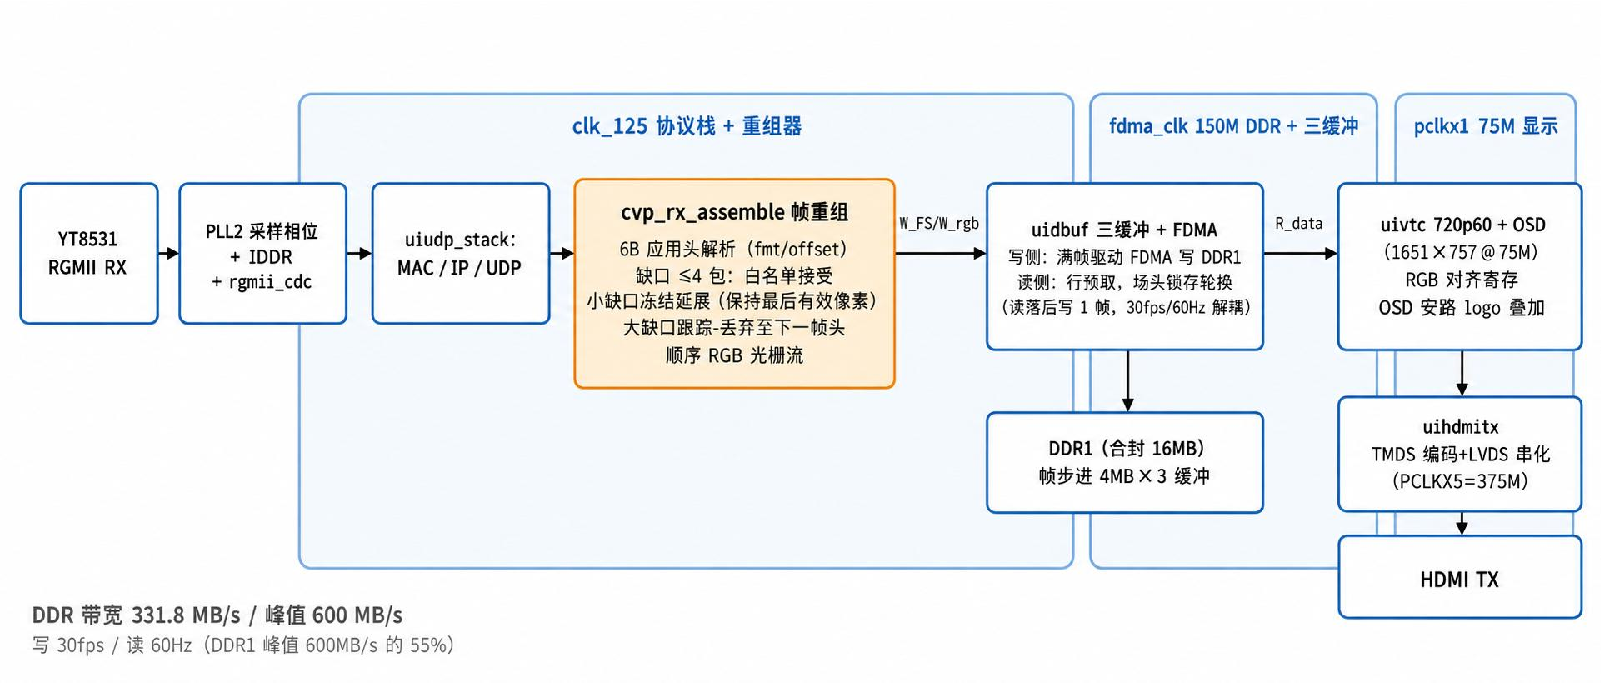
\includegraphics[width=\textwidth]{figs/fig_subboard.pdf}
\caption{子板数据通路:三个时钟域与帧重组/三缓冲/显示输出}
\label{fig:subboard}
\end{figure}

协议栈沿用厂商 UDP 例程(27 文件),其中 MAC 接收层有一处有意修改:广播分支由
"仅 ARP 放行"改为"ARP 或 IP 均放行"(视频流目的 MAC 为广播),IP 层仍有目的
地址精确过滤兜底。本地 IP 设为视频流的目的地址(192.168.1.100),端口 6000 收
视频、6002 状态包按格式字节丢弃。

\section{帧重组器 cvp\_rx\_assemble}

帧重组器是子板的核心自研模块,解决的问题:协议栈输出"无反压、按包到达顺序"的
UDP 载荷字节流,而三缓冲写侧需要"每帧恰好 921{,}600 像素、帧同步脉冲分隔"的
顺序视频流——两者之间隔着丢包、乱序容忍与速率整形三道鸿沟。算法为 PC 收图脚本的
硬件化,适配无反压约束:

\begin{enumerate}[nosep]
\item \textbf{输入侧}(每输入字节 1 拍):解析 6 字节应用头,判定接受条件为
"格式 = 视频 且 偏移 + 1440 $\leq$ 帧长 且(偏移 = 0 新帧标记,或偏移 $\geq$
已承诺位置 且 缺口 $\in\{0,1,2,3,4\}\times$1440B 白名单)"。白名单归纳保证接受
的包恒为整包对齐。接受的包:载荷压入 4096B staging FIFO,描述符(目标偏移)入
8 深队列;偏移为 0 的包先额外插入一条帧尾描述符。
\item \textbf{输出侧}(描述符状态机,严格顺序):S\_FILL 从已输出位置到本描述符
偏移,用最后一个有效 RGB 像素冻结延展,完成缺口对齐;S\_DATA 从 staging 弹 3 字节拼
RGB 输出 480 像素;S\_FS(帧尾描述符)也用最后有效像素延展到帧尾,再发帧同步并清零
位置。
\item \textbf{不变量}:任意两个帧同步脉冲之间恰好输出 921{,}600 像素(实像素 +
冻结延展像素)——保证写侧 FDMA 每帧固定突发数、永不因短帧卡死。
\item \textbf{丢包行为}:连续缺失 $\leq$4 包时接受后续包,缺口以最后有效像素冻结
延展;缺口 $>$4 包时跟踪并丢弃当前帧剩余数据,直到下一帧偏移 0 自动重新同步,
上一帧余量仍由最后有效像素延展;码流彻底中断则最后一完整帧静止显示。
\item \textbf{跟踪-丢弃}:帧尾/洞填充期间(最长约 74 万拍)staging 无法排空,被
水位挡住但通过格式/界内/顺序检查的包\textbf{推进已承诺位置、不入队},避免
committed 停滞引发缺口级联;填充结束即重新同步,损失只限丢包当帧。
\item \textbf{staging 水位论证}:冻结延展期输出 1 像素/拍,对输入 1B/拍,峰值约
2 包(2.9KB)< 4096B;数据期弹 3B/拍 $\geq$ 入速,迅速回落。
\end{enumerate}

\section{DDR 三缓冲与显示输出}

写侧 30\,fps 与读侧 60\,Hz 异步解耦由三缓冲完成:uidbuf 以"写满整帧驱动 FDMA
写、读侧行预取 FDMA 读"的方式访问合封 DDR1(16MB,帧步进 4MB $\times$ 3 缓冲),
场头锁存切换缓冲、读落后写一帧。带宽核算:写 110.6 + 读 221.2 = 331.8\,MB/s,
占 DDR1 峰值 600\,MB/s 的 55\%,余量充足;若需进一步降带宽,后备开关为 RGB565
(数据宽度参数化)。显示侧 uivtc 产生 720p60 时序(1651$\times$757@75M),读出
RGB 与数据使能同拍打一拍寄存后送 uihdmitx(TMDS 编码 + LVDS 串化,
PCLKX5 = 375M);右上角叠加安路 logo OSD(16384$\times$9 位图 + 125 色调色板,
readmemh 初始化)。

\section{时钟与资源}

全板 6 个时钟域:clk\_125(协议栈+重组器)、gmii\_rxc/PLL2(PHY 接收,rgmii\_cdc
跨出)、fdma\_clk 150M(DDR+三缓冲)、pclkx1 75M(显示)、pclkx5 375M(串化
原语内部)、clk\_12\_5(PHY 复位时序);4 个 PLL 全部占用(器件上限 4),时钟组
在 SDC 中显式声明。RGMII 采样相位由 PLL2 CPHASE 控制——采样相位随电源状态漂移
是偶发丢包的根源,诊断 LED 直接指示 CRC 状态,配合 CPHASE 盲扫脚本可求稳定采样
点。资源占用:LUT 7556/19600(38.9\%)、BRAM 44/64。

\section{验证体系}

子板建立三层仿真回归(\verb|tools/sim/|,Python 生成含正确 CRC 的 RGMII 线上
向量注入,期望光栅逐字节比对):\textbf{协议/重组场景回归}(8 场景:完整/丢 1 包/
整帧丢/重复/乱序/坏 FCS/缺 6 包/心跳,8/8 通过);\textbf{全分辨率真机工况回归}
(1920 包/帧 $\times$ 11 帧逐字节比对);\textbf{专项压力测试}(DDR 仲裁 + 刷新
压力扫描、OSD 落点账本逐像素 diff = 0,含 2\,ms 总线黑窗注入的仲裁鲁棒性验证)。
上板验收:HDMI 显示正常、logo 正常;偶发丢包造成的瞬时冻结带由缺口冻结延展缓解
(旧版实现曾以黑色填充,当前版本改为保持最后有效像素)。

\chapter{应用:血细胞形态学检测}
\oneline{在已上板验证的双板相机底座上,以"级联检测"架构把商用形态学分析仪
"检出—分类"链路中的检出半程移入千元级国产 FPGA:前端负责框选、裁剪、上传
(确定性毫秒级,上行链路已由千兆 UDP 实现),上位机负责细分类与图库陈列。
\textbf{本章为应用设计章:检测类新增功能尚未实施,全部指标为设计目标并注明依据。}}

\section{背景与临床价值}

血细胞形态学检查(白细胞五分类计数,原始细胞、浆细胞、有核红细胞等异常细胞的检出)
是血液病筛查的核心手段,当前两端都有痛点:人工镜检慢(每片数十分钟)、依赖经验、
主观差异大;自动化形态学分析仪(CellaVision 及国产同类)检出与分类全自动,但设备
数十万元级,难以在基层普及。任务可以拆成"找细胞"与"认细胞"两半——前者只需要几何与
颜色特征(染色后白细胞核深染、体积大、密度低,经典图像处理即可高召回定位),后者必须
神经网络(核形、颗粒、核浆比等语义特征)。这两半恰好对应"廉价实时硬件"与"通用算力"
的最优分工。

本系统的检测对象是 \textbf{Giemsa(瑞氏—吉姆萨)染色血涂片}:血液推片经甲醇固定后,
以含天青与伊红的 Romanowsky 类染液染色——细胞核、核染质等嗜碱性结构被染成蓝紫色,
血红蛋白与胞浆等嗜酸性结构被染成粉红色。染色后,白细胞核深染、体积明显大于红细胞与
血小板,与背景形成稳定的"颜色—尺寸"对比;中性粒/淋巴/单核/嗜酸/嗜碱五类白细胞亦依
核形与颗粒着色得以区分。这一对比正是"找细胞"可以交给经典图像处理的物理基础:
FPGA 以核深染条件二值化提出候选,实时框选染色细胞,再按框裁剪 96$\times$96 细胞
截图,经千兆网送上位机细分类。

\section{级联检测架构}

前端(FPGA)负责框选、裁剪、上传——哑而快、确定性毫秒级;上位机(PC)负责细分类
与图库展示——算力充足、可迭代升级。这与商用系统的成熟形态一致,本方案的创新点在于
\textbf{把"找"的一半放进百元级国产 FPGA 流水线,使单套系统成本下降 1$\sim$2 个
数量级};同时系统上电即跑、检出不依赖 PC,识别结果驱动 IO 报警,构成"采集—处理—
决策—执行"的完整闭环。系统级数据流如图~\ref{fig:apparch} 所示。

\begin{figure}[H]\centering
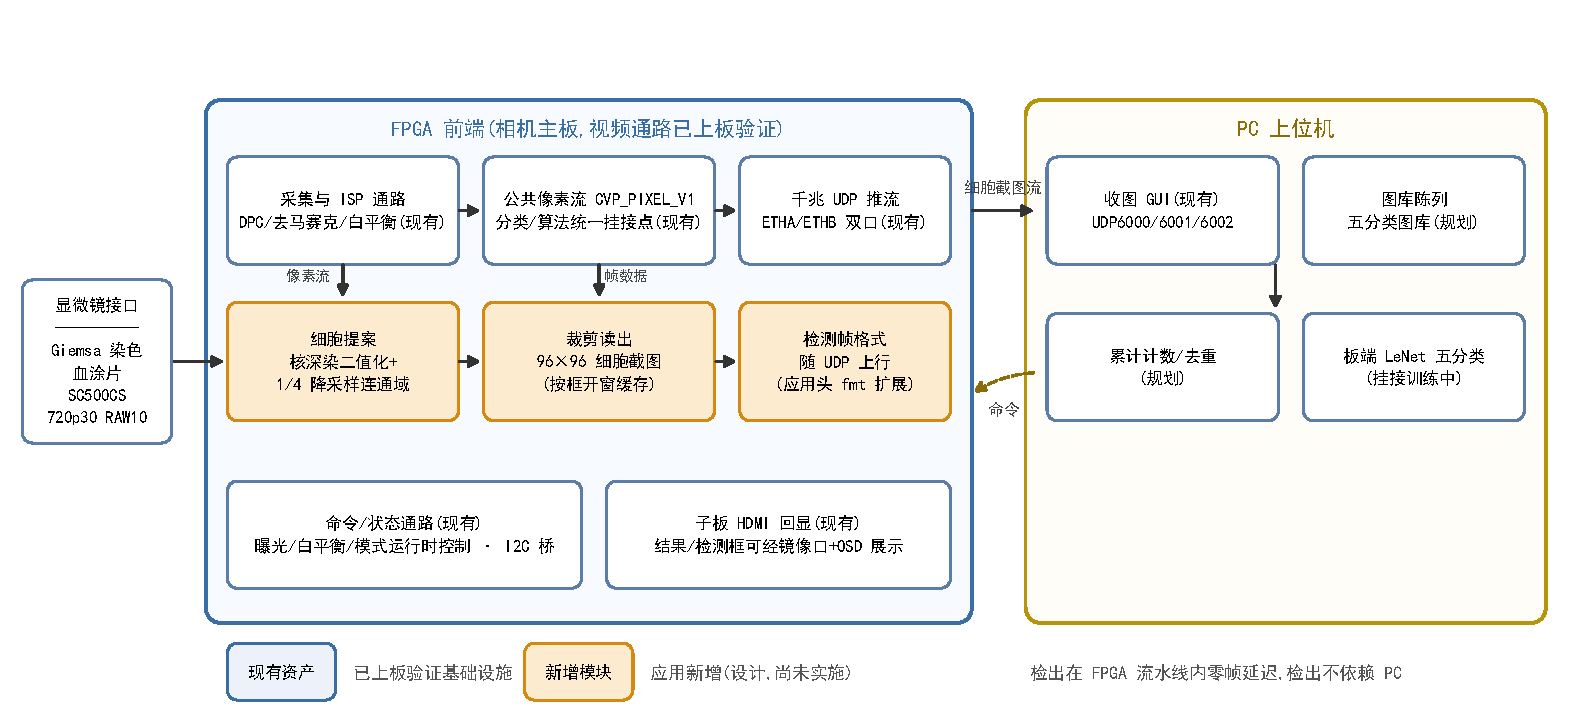
\includegraphics[width=\textwidth]{figs/fig_app_arch.pdf}
\caption{血细胞形态学检测系统级联架构(蓝框 = 已上板验证资产,橙框 = 应用新增模块)}
\label{fig:apparch}
\end{figure}

\section{FPGA 侧新增工作量}

在定版底座上,工程量集中在两个新增 RTL 模块(细胞提案、裁剪读出),上行链路已由
千兆 UDP 推流实现,其余全部复用现有设施:

\begin{table}[h!]\centering\small
\caption{FPGA 侧新增工作量}
\begin{tabular}{p{2.6cm}p{9.2cm}p{2.6cm}}
\toprule
模块 & 做法 & 资源估计 \\
\midrule
细胞提案 & 核深染条件二值化(现有二值化模式改造) $\to$ 1/4 降采样域单趟连通域标记
(标签表存 ERAM) $\to$ 面积/圆度门限筛选 & $<$5\% LUT + 数块 ERAM \\
裁剪读出 & 第 $k$ 帧锁存框坐标 $\to$ 在直通链路上按框开窗缓存 96$\times$96 像素
(行/列计数命中窗口) $\to$ 检测帧格式随 UDP 上行 & 复用为主 \\
去重触发 & 质心注册表自动去重;演示阶段可按键触发整批上传(零逻辑) & $<$1\% LUT \\
\bottomrule
\end{tabular}
\end{table}

\section{复用资产映射}

定版的每一块基础设施在这个应用里都有明确落点,这是"级联架构工作量可控"的依据:

\begin{table}[h!]\centering\small
\caption{复用资产映射(定版底座)}
\begin{tabular}{p{5.4cm}p{9cm}}
\toprule
现有资产 & 在应用中的角色 \\
\midrule
全视频通路(DPC/去马赛克/色彩校正,位级与上板验证) & 提案与裁剪的数据来源,不需要改动 \\
公共像素流接口(CVP\_PIXEL\_V1) & \textbf{分类网络的统一挂接点}:128\,bit 像素字
含坐标/帧身份/模式号元数据,即插即用不动主链路 \\
千兆 UDP 推流(UDP 6000,1920 包/帧)+ ETHA/ETHB 双口 & 裁剪细胞截图与检测结果
的上行链路,\textbf{已实现};检测结果亦可经镜像口驱动子板 OSD 展示 \\
命令/状态通路(UDP 6001/6002) & 曝光/白平衡运行时控制已实现;检测帧格式可在此
扩展 \\
PC 预览 + 子板 HDMI 回显 & 两路并行观察视野(PC/显示器);主板本地 DSI 支路已于 v30 裁剪 \\
二值化等像素级模式 & 细胞提案(核深染掩膜)的实现基础 \\
按键模式切换 & 扫描触发、批管理的人机接口 \\
仿真回归体系(主板 RTL/Python + 子板记分板) & 新增模块沿用同一验证方法论 \\
\bottomrule
\end{tabular}
\end{table}

\section{上位机与分类器}

上位机经网口收包、重组裁剪图,送分类器后在图库 UI 陈列(参考商用形态:左侧实时
视野、右侧分类图库、底部累计计数),并做跨视野去重;收图 GUI 与命令/状态链路
(UDP 6000/6001/6002)已随主板工程交付。分类器目标为板端部署的 LeNet 架构轻量级神经
网络:网络轻量、算力与存储开销低;能否与当前主板工程的剩余资源及时序预算相匹配
仍需在接入真实模型后重新综合、布线和评估,完成五种白细胞的图像
分类;分类挂接点即公共像素流接口(CVP\_PIXEL\_V1),训练以 PBC 公开数据集
(Acevedo 等,约 1.7 万张已裁剪单细胞图、8 类)为起点,再用自采染色图微调。
该方案另有一个数据集红利:FPGA 的裁剪输出天然构成"位置已标定"的细胞图库,
随使用持续积累训练数据。

\needspace{10\baselineskip}
\section{关键指标(设计目标)}

\textbf{下表全部为设计目标与文献依据,不是实测结果}:提案召回阈值将在阶段 0 用 BCCD
数据集仿真标定,分类精度按文献口径,带宽按千兆链路核算。

\begin{table}[H]\centering\small
\caption{关键指标(设计目标)}
\begin{tabular}{p{3.2cm}p{6.4cm}p{4.6cm}}
\toprule
维度 & 指标(目标) & 依据 \\
\midrule
检出实时性 & 30\,fps 流水线内完成,零帧延迟 & 提案在 100\,MHz 写侧流水线内,
1 像素/拍 \\
上传带宽 & 裁剪 96$\times$96 RGB = 27.6\,KB;千兆 UDP 每秒上千张 & 推流链路
实测 1920 包/帧稳定 \\
单张端到端延迟 & $\leq$0.4\,s(检出 0 + 裁剪 $\leq$1 帧 + 传输 + 分类 $<$50\,ms) &
静态视野场景 \\
扫描规模 & 每视野 5$\sim$15 个白细胞;累计 200 个约 1$\sim$2 分钟 & 与商用系统演示
节奏一致 \\
提案召回 & 目标 $\geq$95\%(阈值换召回,误报由上位机分类器剔除) & BCCD 数据集仿真
验证 \\
分类精度 & 主类(五分类)$\geq$95\% & PBC 数据集文献 \\
FPGA 资源 & 与 LeNet 轻量网络共占空闲资源,仍待实现后核算 & v38 主板布线
占用 Slice 10944/21216 (51.58\%),ERAM 51/108、DSP 16/40;可用余量不得直接等同于
可用于网络的预算,接入模型后必须重新评估资源与时序 \\
\bottomrule
\end{tabular}
\end{table}

\needspace{10\baselineskip}
\section{风险与对策}

\begin{table}[H]\centering\small
\caption{风险与对策}
\begin{tabular}{p{3.4cm}p{2.6cm}p{8.2cm}}
\toprule
风险 & 影响 & 对策 \\
\midrule
提案漏检(漏检 = 漏诊) & 系统性 & 阈值放宽换召回 + 面积窗滤血小板簇;BCCD 仿真定
阈值,召回作硬指标验收 \\
色彩保真(分型依赖染色色度) & 分类精度 & 白平衡已支持四模式 + 网络运行时控制
(第 4 章),视野内放白色参考块锚定;进阶:裁剪改传 RAW10(免插值色偏),上位机
统一处理 \\
异常类别训练数据稀缺(原始细胞/浆细胞/有核 RBC) & 扩展受限 & 演示版做五分类 +
"异常可疑"兜底类(低置信度标黄人工复核),异常检出作为扩展方向 \\
30\,fps 推流高带宽占用 & 上传并发 & 检测帧与视频帧分端口/分格式;必要时降帧 \\
\bottomrule
\end{tabular}
\end{table}

\needspace{10\baselineskip}
\section{实施计划}

\begin{table}[H]\centering\small
\caption{实施计划}
\begin{tabular}{cp{7.4cm}p{3.6cm}p{2.4cm}}
\toprule
阶段 & 内容 & 产出/判据 & 状态 \\
\midrule
0 & 软件闭环:BCCD 提案召回实验 + 上位机原型 & 召回率—误报率曲线定阈值;UI 定版 &
AE 控制律/GUI 已完成,余项进行中 \\
1 & FPGA 提案 + 框选 + 计数 & 实时框选白细胞,仿真逐位对拍通过 & 待启动(需板) \\
2 & 裁剪读出 + 千兆上行 + 上位机接通 & 图库逐个生成分类细胞 & 上行链路已就绪 \\
3 & LeNet 五分类 + 累计计数、去重、异常标黄 & 200 细胞累计扫描全流程演示 &
网络训练进行中 \\
4(可选) & 多前端汇聚演示 & 网络化形态 & 规划 \\
\bottomrule
\end{tabular}
\end{table}

\noindent 阶段 0 不需要任何硬件投入,即可验证全部关键假设(召回可达性、阈值、
上位机形态);阶段 1 起依赖上板(部署流程见各工程 README)。

\section{结论}

\textbf{技术可行}:所需算法(二值化/连通域/裁剪/统计)均为 FPGA 流水线的经典问题,
上行链路已在定版中实现,无技术空白点;\textbf{价值成立}:把商用形态学分析仪
"检出—分类"链路中的检出半程移入千元级国产 FPGA,单套成本降 1$\sim$2 个数量级,
且检出部分确定性毫秒级延迟、可 7$\times$24 运行;\textbf{风险可控}:主要风险
(提案召回、色彩保真)均有量化验收手段与既定对策,全部关键假设可在零硬件投入的
阶段 0 先行验证;\textbf{叙事完整}:从"实时视觉前端平台"到"血细胞形态学检测"的
垂直应用,展示同一硬件底座(实时流式处理 + 网络命令控制 + 千兆上行 + 双板三路
显示)的可复用性。


\end{document}
